\section{Truthful Verified Credit}
\label{sec:method}
% With the problem defined in \cref{sec:problem}, we introduce the mechanism of \tvc{}. It has three parts, and each answers one failure of reliance credit mentioned. We first introduce the three components of the proposed mechanism. We then explain how the mechanism addresses the credit assignment problem and why each component is essential. Finally, we illustrate its operation through a simple example.

\subsection{Verified externality credit}
\label{sec:ext}

Popularity credit rewards a fake claim and a real one alike, because both attract followers. Let $\mathcal F_i^t=\{j:\,d_j^t=i\}$ be the \emph{follow set} of sender $i$: the receivers $j$ that follow $i$'s claim in round $t$ and so observe $\theta_i^t$ exactly. \tvc{} instead credits the followers' realized gain \cref{eq:gain}, and only for a claim that is verified:
\begin{equation}
  \sum_{j\in\mathcal F_i^t} V_i^t\,\min\!\big(g_{ji}^t,\,\Bbar\vbar\big).
  \label{eq:ext}
\end{equation}
Here $V_i^t=\mathbb{1}\big[\,|m_i^t/\theta_i^t-1|\le\tau\,\big]$ is the verification gate: it equals $1$ when the claim lies within a tolerance $\tau\ge0$ of the true value $\theta_i^t$, and $0$ otherwise. The tolerance $\tau$ is set above the honest noise level $\epsilon$, so a truthful claim passes the gate and any claim outside the tolerance is blocked. Every $j\in\mathcal F_i^t$ learns $\theta_i^t$ exactly on committing, so a followed claim ($\mathcal F_i^t\neq\emptyset$) is checked at no cost to the designer. 

The gain $g_{ji}^t$ is the externality of $i$'s report on $j$ relative to $j$ staying put, as in a VCG mechanism \citep{vickrey1961counterspeculation,clarke1971multipart,groves1973incentives}. A lie that is followed fails the gate $V_i^t$ and earns no gain credit, so attracting followers with an inflated claim no longer brings a gain. The cap $\Bbar\vbar$, with $\Bbar>0$ a design parameter in units of the mean value $\vbar$, limits what one follower can add, so a single lucky find cannot dominate the sender's return. Each receiver follows at most one claim, so the cap also bounds the cost: the gain term adds at most $N\Bbar\vbar$ per round.

\subsection{Checked score bonus}
\label{sec:bonus}

Gain credit alone leaves silence as a best response: a true claim that nobody follows earns nothing, exactly like staying silent. \tvc{} therefore gives every checked claim a bonus that peaks at the truth,
\begin{equation}
  \chi_i^t\,\eta\,\vbar\,S\big(m_i^t,\theta_i^t\big),
  \label{eq:bonus}
\end{equation}
where $\eta>0$ is the bonus weight and the score is a Gaussian in the log error with width $w>0$,
\begin{equation}
  S(m,\theta)=\exp\!\Big(-\frac{(\ln m-\ln\theta)^2}{2w^2}\Big).
  \label{eq:score}
\end{equation}
A claim is \emph{checked} when it is audited or followed,
\begin{equation}
  \chi_i^t=\mathbb 1[m_i^t\neq\varnothing]\,\max\big(a_i^t,f_i^t\big),
  \qquad
  f_i^t=\mathbb 1\big[\mathcal F_i^t\neq\emptyset\big],
  \label{eq:checked}
\end{equation}
where $f_i^t$ indicates that someone followed $i$, and $a_i^t$ indicates a random audit of the claim, drawn independently of the claim and of the receivers,
\begin{equation}
  a_i^t\sim\mathrm{Bernoulli}(p),\qquad p\in(0,1].
  \label{eq:audit}
\end{equation}
A claim is thus checked either by a follower or by a random audit, and the audit is what reaches claims nobody follows. Because the audit is independent of the claim and of the receivers, a true claim earns at least $p\,\eta\vbar$ in expectation however receivers behave, and this is strictly more than silence, which earns $0$. This holds for a bad find as well, so reporting a low-value find is no longer a loss. The score is $1$ at the truth and below $\sbar=\sup_{|m/\theta-1|>\tau}S(m,\theta)<1$ for every claim that fails the tolerance, so inflation cannot raise the bonus.

\subsection{Audited lying cost}
\label{sec:cost}

The first two parts leave a lie with a small payoff, the bonus up to $\eta\sbar\vbar$, and say nothing about an outside gain $\Gamma$, the net private benefit a lie brings its sender outside the credit channel, for example a false report that steers others away from something the sender wants for itself. \tvc{} therefore fines every audited claim that fails verification, with a fine $\varphi\ge0$ in units of $\vbar$:
\begin{equation}
  a_i^t\,(1-V_i^t)\,\mathbb 1[m_i^t\neq\varnothing]\,\varphi\,\vbar.
  \label{eq:cost}
\end{equation}
The fine is charged only on audits. An audit has probability $p$, independent of the claim and the receivers, so a lie costs $p\varphi\vbar$ in expectation whatever the receivers do, and the fine can be sized against $\Gamma$ without a model of the receivers (\cref{eq:fine}). Raising $\varphi$ lets the designer lower the audit rate $p$, which is the price of verification. We do not assume limited liability, so the net credit may be negative.

% We do not need to audit every claim. In an allocation problem with costly verification, \citet{benporath2014OptimalAllocationCostly} show that when lying carries a cost $\varphi$, the optimal mechanism is still a favored-agent mechanism, but its checking probability falls from $1$ to $1/(1+\varphi)$.


Together, the credit to sender $i$ in round $t$ is
\begin{equation}
  \begin{aligned}
    C_i^t ={}& \textstyle\sum_{j\in\mathcal F_i^t} V_i^t \min\!\big(g_{ji}^t,\Bbar\vbar\big) \\
    &+ \chi_i^t\,\eta\,\vbar\, S\big(m_i^t,\theta_i^t\big) \\
    &- a_i^t\big(1-V_i^t\big)\mathbb{1}\big[m_i^t\neq\varnothing\big]\,\varphi\,\vbar .
  \end{aligned}
  \label{eq:tvc}
\end{equation}
% \tvc{} wraps any existing credit scheme: the host's credit for a claim is replaced by \cref{eq:tvc}.

The algorithm for learning with \tvc{} per episode is shown in \cref{alg:tvc}, and the credit of one claim in \cref{alg:credit}.




% \begin{figure*}[t]
%   \centering
%   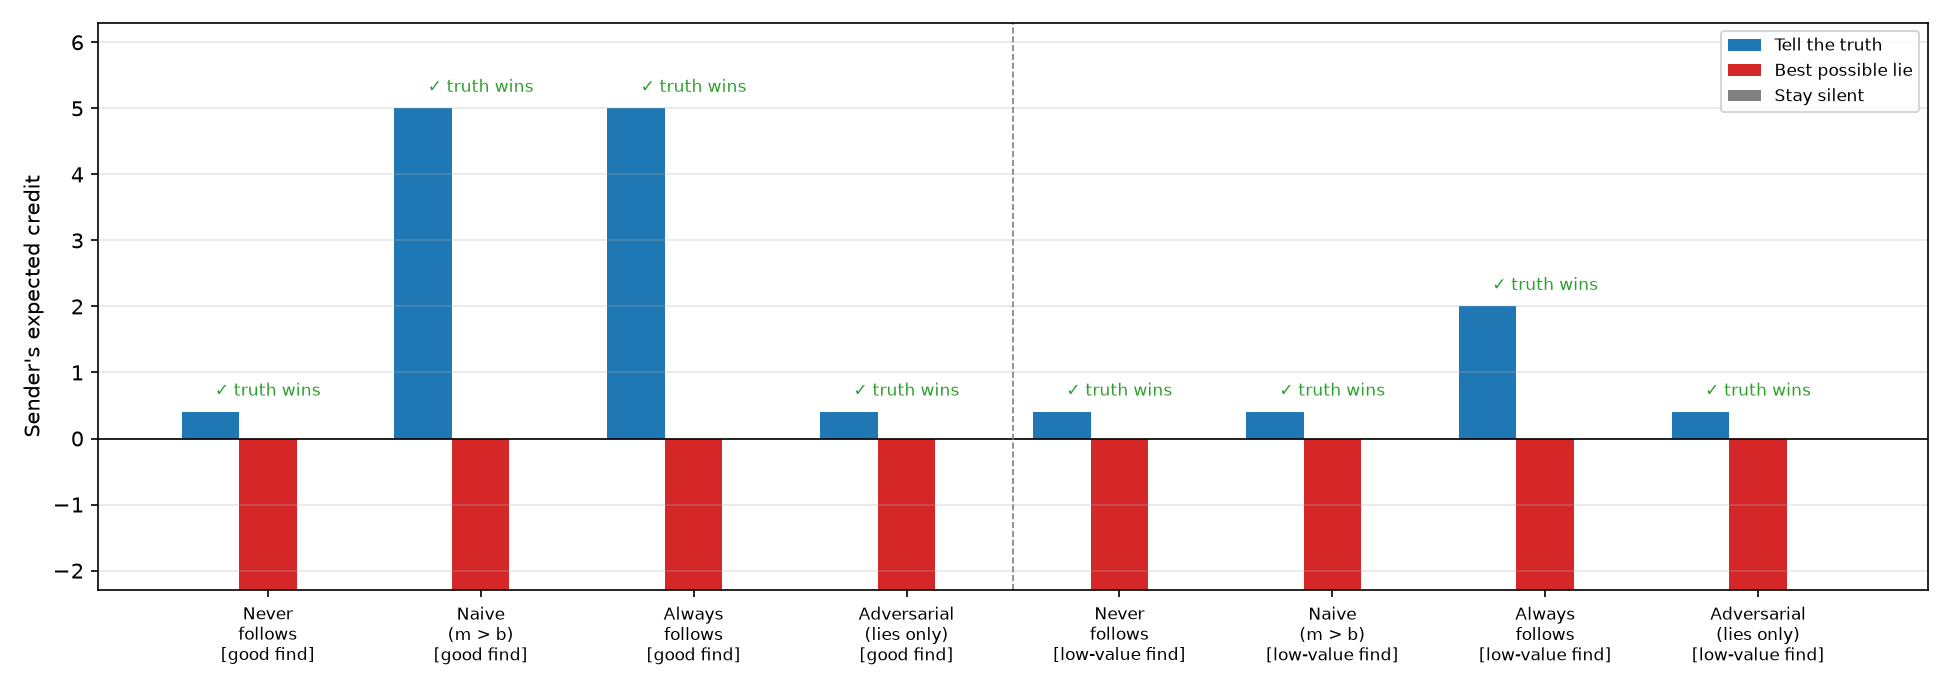
\includegraphics[width=\textwidth]{figures/honesty_every_case.png}
%   \caption{Truth against the best lie and silence under \tvc{}, for one sender, one receiver and one round. Each pair of groups of bars is a receiver rule (never follows, follows if the claim beats its best, always follows, or follows only lies) for a good find ($\theta=2$) and for a low-value find ($\theta=0.8$), with the follower's best value at $1$. Blue is the expected credit of the truthful claim, red is the best of the lies $\times0.9$, $\times1.1$, $\times1.5$ and $\times2$, and grey is silence, which earns $0$. Credit is in units of $\vbar$ and expected over the audit ($p=0.2$). Truth earns more than every lie and than silence in all eight cases.}
%   \label{fig:every_case}
% \end{figure*}

% \paragraph{Outside gain.}
% A lie can also be profitable for reasons outside the credit, a private gain $\Gamma$ that the designer neither observes nor rewards (defined in \cref{app:fine}). Truth then stays strictly dominant only if the fine exceeds $\philo=(\eta\sbar+\Gamma)/p-\eta$ (\cref{eq:fine}). A larger outside gain needs a larger fine, and so do fewer audits, in proportion to $1/p$.

% ---------------------------------------------------------------------------------------------------
\subsection{When \tvc{} is useful}
\label{sec:when}

\tvc{} is aimed at settings where four conditions hold together.
\begin{enumerate}
  \item \emph{Credit follows reliance.} Agents are credited for being followed or used, which rewards exaggeration and leaves a true report that nobody uses uncredited.
  \item \emph{Lying is profitable outside the credit.} Agents are not fully prosocial ($\lambda<1$), so a lie can bring a private gain that no reliance credit removes by itself.
  \item \emph{Lying harms others.} A false report misleads those who act on it and wastes their effort, and the group loses once several agents lie. Where receivers can decode exaggeration at little cost, hype costs little, and \tvc{} buys honest reports but not extra welfare.
  \item \emph{Claims can be audited at a cost.} Receivers cannot verify a claim before acting, but the designer can check a random sample at rate $p$.
\end{enumerate}
One of our testbeds meets all four (\cref{sec:experiments}). Other candidates, which we do not evaluate, are crowd-sourced traffic or robot-fleet reports, teams of language-model agents that build on one another's findings, and scientific credit through citations with sampled replication as the audit. When a condition fails, simpler designs may suffice: a shared return can work for nearly altruistic agents, and without any audit, peer prediction is the relevant regime.

% ---------------------------------------------------------------------------------------------------
% Job: make it implementable in a few lines. The credit of each claim is added to the return of the decision that
% produced it; everything else in the learner is unchanged.

\begin{algorithm}[t]
  \caption{Learning with \tvc{} (per episode)}
  \label{alg:tvc}
  \begin{algorithmic}
    \STATE Each sender decides to post a claim $m_i^t$ or stay silent; draw an audit $a_i^t\sim\mathrm{Bernoulli}(p)$ per claim
    \STATE Receivers act on the claims by their own rule; record who relied on which claim
    \STATE Mark a claim checked if it was audited or its outcome was observed by someone who relied on it
    \FOR{each claim}
      \STATE Compute $C_i^t$ by \cref{alg:credit}
      \STATE Add $C_i^t$ to the return of the decision that posted the claim
    \ENDFOR
    \STATE Update each sender's policy with its usual learning rule
  \end{algorithmic}
\end{algorithm}

\begin{algorithm}[t]
  \caption{\tvc{} credit of one sender in one round (the credit step of \cref{alg:tvc})}
  \label{alg:credit}
  \begin{algorithmic}
    \REQUIRE claim $m_i^t$ or silence $\varnothing$; follow set $\mathcal F_i^t$ and gains $g_{ji}^t$; audit draw $a_i^t$; true value $\theta_i^t$, revealed by a check; parameters $\tau,\Bbar,\eta,w,\varphi$
    \ENSURE credit $C_i^t$
    \IF{$m_i^t=\varnothing$}
      \STATE \textbf{return} $0$
    \ENDIF
    \STATE $\chi_i^t\leftarrow\max\big(a_i^t,\ \mathbb 1[\mathcal F_i^t\neq\emptyset]\big)$ \COMMENT{checked by an audit or a follower}
    \IF{$\chi_i^t=0$}
      \STATE \textbf{return} $0$ \COMMENT{an unchecked claim earns nothing}
    \ENDIF
    \STATE $V_i^t\leftarrow\mathbb 1\big[\,|m_i^t/\theta_i^t-1|\le\tau\,\big]$ \COMMENT{verification gate}
    \STATE $C_i^t\leftarrow\eta\,\vbar\,S\big(m_i^t,\theta_i^t\big)$ \COMMENT{score bonus}
    \IF{$V_i^t=1$}
      \STATE $C_i^t\leftarrow C_i^t+\sum_{j\in\mathcal F_i^t}\min\big(g_{ji}^t,\Bbar\vbar\big)$ \COMMENT{verified gain credit}
    \ELSIF{$a_i^t=1$}
      \STATE $C_i^t\leftarrow C_i^t-\varphi\,\vbar$ \COMMENT{fine for an audited false claim}
    \ENDIF
    \STATE \textbf{return} $C_i^t$
  \end{algorithmic}
\end{algorithm}

\todo{Parameter recipe: $\eta$ and $\Bbar$ in units of the mean value $\vbar$; $p$ from the audit budget; $\varphi = 2\philo$ from \cref{eq:fine}. Cost: one audit per $1/p$ claims.}
